\documentclass{article}
\usepackage[utf8]{inputenc}
\usepackage[hidelinks]{hyperref}
\usepackage[spanish]{babel}
\usepackage[left=2cm,right=2cm,top=2cm,bottom=2cm]{geometry}
\usepackage{graphicx}
\usepackage{pdflscape}
\usepackage{listings}

\lstset {
    frame = single,
    breaklines = true
}

\begin{document}
\begin{titlepage}
\title{\textbf{
    {\Huge Práctica 4: Métodos Lineales de Regresión y Clasificación}\\
    {\Large Almacenes y Minería de Datos}
}}
\author{
    Pedro Allué Tamargo (758267)
    \and
    Cristina Oriol García (755922)
    \and
    Alejandro Paricio García (761783)
}
\date{\today}
\clearpage\maketitle
\thispagestyle{empty}
\end{titlepage}

% Index
\tableofcontents

\newpage
\section{Introducción}

En esta práctica se van a utilizar los conceptos de regresiones lineales y logísticas vistos en clase. Estos conceptos son muy útiles de cara al cálculo de predicciones. En el caso de las regresiones lineales se van a utilizar para estudiar qué compuestos son importantes en los análisis de los antioxidantes para 5 variables de las cervezas. En el caso de las regresiones logísticas se utilizarán para estudiar el comportamiento de unos fardos de droga que son tirados al mar por los narcotraficantes y van a parar a 3 calas distintas dependiendo de la posición desde la que se lanzan.\\

\newpage
\section{Problema 1}
\subsection{Análisis de los ensayos}

\subsubsection{Análisis variable \textit{DSA}}

Se ha creado un modelo de regresión lineal utilizando las variables \textit{tpc}, \textit{tso2} y \textit{ma}. Se puede observar que en la salida obtenida para este modelo (Figura \ref{fig:dsa_3_variables}) el \textit{p-valor} del \textit{F estadístico} tiene un valor por debajo de \textit{0.05} y por lo tanto implica que $\exists \hat{\beta_i}\neq0$. Esto implica que alguno de los estimadores $\beta$ es influyente en el modelo. Utilizando las 3 variables se obtiene un \textit{adjusted $R^2$} que explica el $69\%$ de la varianza.\\

Se va a proceder a realizar otro modelo de regresión lineal descartando la variable \textit{ma}. Se ha descartado esta variable porque su \textit{p-valor} es muy alto con respecto al de los demás predictores. La salida obtenida con este modelo se puede observar en la Figura \ref{fig:dsa_2_variables}. Se puede observar que el \textit{p-valor} del \textit{F estadístico} sigue siendo inferior al umbral (\textit{0.05}) y por lo tanto existe algún predictor que es influyente en el modelo. Tambíen se puede observar que el \textit{adjusted $R^2$} ha aumentado (\textit{60\%}). Ha subido al eliminar el preditor \textit{ma} debido a la penalización asociada de aumentar el número de predictores no influyentes.\\

Tras concluir que al menos un elemento es influyente en el modelo se va a analizar con únicamente el predictor \textit{tpc}. Los resultados de este modelo se pueden encontrar en la Figura \ref{fig:dsa_1_variable}. Se puede observar que el \textit{adjusted $R^2$} baja respecto al análisis anterior a explicar solamente el 68\% de la varianza. Esto implica que la variable \textit{tso2} era influyente en cierta medida pero menos que la variable \textit{tpc}. El \textit{p-valor} sigue siendo menor que $0.05$ y por lo tanto implica que la variable \textit{tpc} es influyente ($\hat{\beta_{tpc}}\neq0)$.\\

Para concluir, se va a proceder a crear un modelo de regresión lineal utilizando la variable \textit{tso2}. Los resultados se pueden observar en la Figura \ref{fig:dsa_1_variable_tso2}. Se puede observar que el \textit{p-valor} tiene un valor superior a $0.05$ y por lo tanto se acepta la hipótesis nula que dice que $\hat{\beta_{tso2}}=0$. La conclusión de este análisis es que la variable \textit{tso2} influye muy poco sobre el modelo con respecto a la variable \textit{tpc}.\\

Partiendo de los modelos anteriores se ha llegado a la conclusión de que los predictores \textit{ma} y \textit{tso2} no son suficientemente influyentes, por lo que la variable \textit{dsa} quedaría explicada únicamente con \textit{tpc}. El descarte de \textit{ma} es claro, no obstante, el de \textit{tso2} no lo es tanto. Primero se observó que influía en cierta medida, ya que al incluirlo se pasaba de explicar el 68\% al 70\% de la variabilidad. Pese a ello, al observar cómo explicaba por si mismo \textit{tso2} a \textit{dsa}, el análisis de los resultados daba a entender que no era influyente. El balance entre ambas posibilidades llevó a la eliminación del predictor anterior en este tipo de examen de propiedades antioxidantes.\\


\subsubsection{Análisis variable RP}

Se ha realizado un primer análisis sobre la variable \textit{RP} utilizando las 3 variables (Figura \ref{fig:rp_3_variables}). Se puede observar que el \textit{p-valor} de la variable \textit{ma} es superior a los anteriores y eso puede significar que no sea influyente en el análisis. El modelo tiene un \textit{p-valor} en el F estadístico muy bajo (inferior a \textit{0.01}) y por lo tanto implica que $\exists\hat{\beta_i}\neq0$, es decir, alguno de los estimadores parece tener influencia en el modelo. El \textit{adjusted $R^2$} presenta un valor de \textit{56\%}. Esto implica que el modelo con los predictores actuales explica un 56\% de la varianza.\\

Dado que la variable \textit{ma} ha mostrado un \textit{p-valor} alto se va a proceder a realizar otro modelo de regresión lineal sin utilizar esta variable. En la Figura \ref{fig:rp_2_variables} se puede observar el resultado de este modelo. Se puede observar que el modelo sigue presentando un \textit{p-valor} en el \textit{F estadístico} muy pequeño, por lo tanto implica que $\exists\hat{\beta_i}\neq0$, es decir, alguno de los estimadores tiene influencia en el modelo. Se puede observar que el \textit{adjusted $R^2$} presenta un valor mínimamente superior al obtenido en el modelo de 3 variables (Figura \ref{fig:rp_3_variables}). Esto se debe a que al eliminar una variable que no influía sobre el modelo se reduce la penalización del número de variables en el modelo.\\

Puesto que la variable \textit{tso2} presenta un \textit{p-valor} superior al presentado por la variable \textit{tpc} pero inferior al umbral \textit{0.05} se va a proceder a realizar un modelo con el cual solo se tenga en cuenta la variable \textit{tpc}. El resultado de este modelo se puede observar en la Figura \ref{fig:rp_1_variable_tpc}. Se puede observar que el \textit{p-valor} del \textit{F estadístico} tiene un valor muy próximo a \textit{0} y menor que el umbral \textit{0.01} y por lo tanto existe un estimador que es influyente en el modelo. En este caso, al solo contar con la variable \textit{tpc} se puede llegar a la conclusión de que esta variable es influyente en el modelo. También se puede observar que el valor de \textit{adjusted $R^2$} se ha reducido ligeramente comparado con el modelo de la Figura \ref{fig:rp_2_variables} ya que ha pasado del valor \textit{57\%} a un \textit{53\%}. Esto implica que la variable \textit{tso2} era influyente en el modelo aunque no tanto como \textit{tpc}.\\

Para comprobar la hipótesis de que la variable \textit{tso2} es influyente en el modelo se va a realizar un modelo utilizando solo esa variable para intentar predecir el valor de la variable \textit{RP}. Los resultados de este modelo se pueden observar en la Figura \ref{fig:rp_1_variable_tso2}. Se puede observar que el \textit{p-valor} del \textit{F estadístico} es menor que un umbral de \textit{0.05} y próximo al umbral de \textit{0.01} y por lo tanto la variable \textit{tso2} es influyente en el modelo. También se puede observar que el \textit{adjusted $R^2$} indica que esta variable es capaz de explicar un \textit{13\%} de la varianza.\\

Por lo tanto, se puede concluir que las variables \textit{tpc} y \textit{tso2} son influyentes en el modelo de regresión lineal para el antioxidante \textit{RP}. La variable \textit{tso2} no es tan influyente en el mismo como la variable \textit{tpc}.\\


\subsubsection{Análisis variable ORAC}

El primer paso es llevar a cabo la regresión lineal sobre la varrable ORAC utilizando \textit{tsp}, \textit{tso2} y \textit{ma}. La figura \ref{fig:orac_3_variables} muestra los resultados. Se puede observar que el $R^{2}$ adquiere un valor muy bajo, explicando únicamente el 20\% de la varianza. Además, el p--valor del F--estadístico tiene un valor de 0.042, bastante superior a 0.01, lo que nos indica que es muy probable que no haya ningún predictor realmente influyente en el modelo. Si estudiamos los p--valores de cada uno de los predictores podemos descartar directamente \textit{tso2} y \textit{ma}. Debido a ello, se va a analizar el modelo con únicamente la variable tpc, los resultados se pueden observar en la figura \ref{fig:orac_1_variable_tpc}.\\

Vuelven a reportarse p--valores cuestionables para \textit{tpc}. El p--valor del F--estadístico no es suficientemente bajo como para determinar que con alta probabilidad alguno de los predictores es influyente, y la varianza explicada ronda el 12\%. Se puede concluir que, pese a que \textit{tpc} es la que más contribuye a la explicación de \textit{orac} de entre las tres, no se puede garantizar que sea suficientemente influyente como para llegar a ser relevante sino que, más bien contrario, su p--valor parece indicar que no es lo suficientemente bueno. Es el único predictor restante, eliminarlo daría lugar a tener en cuenta únicamente el interceptor, que tomaría como valor la media de los datos. Los resultados de esto se muestran en la figura \ref{fig:media_orac}. Estos confirman la hipótesis anterior de que no era lo suficientemente relevante y apoya la idea extraída a partir del primer p--valor del F--estadístico, que indicaba que era muy probable que ninguno de los predictores fuera distinto de cero. \\

Se concluye que \textit{tpc} influye muy poco en el resultado y que en ningún caso se explica suficientemente bien la varianza de los datos. Esto nos indica que éstos no son predictores del todo apropiados del test ORAC, lo que puede abrir la pregunta acerca de la corrección del estudio del problema, puesto que podrían estar pasándose por alto otros factores que si que sean influyentes en el anterior y que deberían considerarse.


\subsubsection{Análisis variable ASA}

Primero llevamos a cabo una regresión lineal utilizando las tres variables \textit{tpc, tso2, ma}. Como se muestra en la figura \ref{fig:asa_3_variables} podemos ver que el $R^{2}$ tiene un valor bastante lo que significa que solo explica un 22\%de la varianza. Observamos que el p--valor de F--estadístico tiene un valor de 0.0067 por lo que podemos suponer que alguna de los predictores influye en el modelo. Analizando los valores de estos predictores podemos observar que el p--valor de \textit{ma, tso2} es excesivamente alto por lo que podemos descartarlos de este modelo. \\

Por otro lado el p--valor de \textit{tpc} es lo suficientemente bajo como para concluir que es influyente en nuestro modelo. 
Procedemos a hacer un análisis únicamente sobre la variable \textit{tpc} por los datos comentados anteriormente. El resultado lo observamos en la figura \ref{fig:asa_1_variable}. Como se puede observar según el $R^{2}$ se explica un 26\% de la varianza, subiendo respecto al modelo anterior únicamente un 4\%. Tanto el p--valor del F--estadístico como el p--valor del predictor \textit{tpc} mantienen que este predictor influye en nuestro modelo. Aunque sigue sin explicar correctamente la varianza de los datos. \\

Para comprobar las hipótesis sobre los predictores realizamos un último análisis sobre las variables previamente descartadas, podemos ver el resultado en la figura \ref{fig:asa_2_variables} . De este análisis comprobamos que el F--estadístico es 1,41 suficientemente cercano a 1 y su p--valor 0.257 suficientemente grande para concluir que efectivamente los dos predictores utilizados no influyen en nuestro modelo, aceptando la hipótesis nula habiendo optado correctamente por su descarte.\\

De estos análisis podemos concluir que únicamente \textit{tpc} influye en los resultados obtenidos aunque no explica suficientemente la varianza de los datos.


\subsubsection{Análisis variable MCA}

Como podemos observar en la figura \ref{fig:mca_3_variables} el p--valor del F--estadístico nos indica que al menos uno de los predictores influye en el modelo, con la información proporcionada por los p--valor de cada predictor podemos descartar los predictores \textit{ma, tso2} por tener un valor excesivamente alto, por lo que el único con un valor aceptable sería \textit{tpc}. Realizamos un análisis con únicamente este predictor, como se ve reflejado en la figura \ref{fig:mca_1_variable} los p--valores continúan siendo suficientemente pequeños como para determinar que este predictor efectivamente influye en nuestra variable y como nos indica el $R^{2}$ explica un 37\% de la varianza de esta variable.\\


\subsection{Conclusiones del análisis de antioxidantes}

Tras la realización de los análisis de los antioxidantes estudiados anteriormente se puede observar que el compuesto \textit{tpc} es muy influyente en los cinco ensayos. Otro compuesto influyente es \textit{tso2} aunque en menor medida que el \textit{tpc}. El compuesto \textit{ma} no es influyente en ninguno de los ensayos.\\

No obstante, en los ensayos \textit{ORAC}, \textit{ASA}, \textit{MCA} se puede observar que \textit{tpc} da parte de la explicación de la varianza pero no toda y por lo tanto puede existir, o no, algún compuesto más que no se esté teniendo en cuenta en este conjunto de datos.


\newpage
\section{Problema 2}

\subsection{Parte 1: ¿A dónde va el fardo?}

Para la realización de este ejercicio se ha utilizado la interpretación geométrica de las regresiones logísticas. Si se interpreta de que la playa es una línea recta que se describe entre los puntos de mayor y menor latitud entonces los puntos que dividen las zonas de las 3 calas se corresponden con las intersecciones de las rectas creadas por las regresiones logísticas con la recta de la playa. Una representación de esto se puede observar en la Figura \ref{fig:divisionPlayaRectas}.\\
Se puede observar que la recta que describe la playa se corresponde con la recta $y = -1.842551x + 18.711764$.\\

Como nos encontramos ante una recta el uso de los dos parámetros no es necesario ya que al conocer la ecuación de esta teniendo uno de los dos podríamos calcular el otro así que es posible prescindir de uno de los dos, no importa cual para el cálculo del modelo. Si se opta por tener en cuenta los dos se obtiene el modelo que se puede observar en la figura: \ref{fig:modelo_2_param} como se muestra los p--valores de los dos predictores son excesivamente altos por la relación entre ellos previamente comentada, por eso se ha decidido utilizar exclusivamente el parámetro \textit{latitud.y}\\

Para hallar estas dos rectas se han creado dos regresiones logísticas con el objetivo de hallar qué fardos terminarán en la cala 0 y qué fardos terminarán en la cala 2. Por lo tanto dado un punto si estas regresiones predicen una probabilidad cercana a 0 de que el fardo termine en la cala 0 y la cala 2 significará que el fardo terminará en la cala 1.\\

Las rectas correspondientes a los modelos de regresión logística son:
\begin{itemize}
    \item Regresión de \textit{Cala 0}: $y = 0.001563063x + 1.087117$
    \item Regresión de \textit{Cala 2}: $y = -0.001635438x + 1.099433$
\end{itemize}

El código correspondiente a la creación de los modelos se puede encontrar en el \textit{Listing \ref{listing:codigoFardosModelos}}.\\

Los puntos que dividen la playa en las 3 calas se pueden averiguar calculando la intersección de las 3 rectas (regresiones logísticas y playa). El punto de corte situado más al norte (latitud mayor) es: \textit{(9.557243, 1.102056)} y el punto de corte situado más al sur es: \textit{(9.5671585, 1.0837867)}.\\

Para estas funciones se han utilizado los modelos anteriores y mediante una normalización de las probabilidades se han hallado las 3 componentes. Ha sido necesaria la normalización de estos debido a que al utilizar dos regresiones logísticas binomiales las probabilidades para la cala \textit{``pivote''} no se podía obtener el valor realizando una resta con la unidad. La fórmula utilizada para la normalización de las probabilidades de cada una de las variables es\footnote{\url{https://en.wikipedia.org/wiki/Multinomial_logistic_regression#As_a_set_of_independent_binary_regressions}}:

\begin{equation}
    p(cala = 0) = \frac{\frac{P(cala = 0 | modelo = 1)}{P(cala = 1 | modelo = 1)}}{1 + \frac{P(cala = 0 | modelo = 1)}{P(cala = 1 | modelo = 1)} + \frac{P(cala = 2 | modelo = 2)}{P(cala = 1 | modelo = 2)}}\\
\end{equation}

\begin{equation}
    p(cala = 2) = \frac{\frac{P(cala = 2 | modelo = 2)}{P(cala = 1 | modelo = 2)}}{1 + \frac{P(cala = 0 | modelo = 1)}{P(cala = 1 | modelo = 1)} + \frac{P(cala = 2 | modelo = 2)}{P(cala = 1 | modelo = 2)}}
\end{equation}

\begin{equation}
    p(cala = 1) = 1 - (p(cala = 0) + p(cala = 2))
\end{equation}

Para el cálculo de la matriz de confusión de este modelo se ha realizado una partición de los datos utilizando el 80\% para entrenarlo y el resto como test obteniendo los resultados que se pueden encontrar en la figura \ref{fig:matrizConfusion}.\\
Para calcular la probabilidad de que dadas unas coordenadas un fardo aparezca en cada cala se ha combinado el resultado obtenido de las dos regresiones logísticas en una función \textit{calcularProbCala} que devuelve un vector con las tres probabilidades correspondientes. El cálculo de la cala para una coordenada se hace en \textit{caclularCala} utilizando esta función previamente comentada devolviendo como resultado la calla cuya probabilidad sea más alta.\\

Los resultados obtenidos para los tres fardos pedidos han sido:
\begin{itemize}
    \item Primer fardo con coordenadas \textit{(9,558359, 1,1)}: Llega a la cala 2 con una probabilidad: \textit{(0.0001090677 0.414166 0.5857249)} para las respectivas calas.
    \item Segundo fardo con coordenadas \textit{(9,564329, 1,089) }: Llega a la cala 1 con una probabilidad: \textit{(0.2303593 0.7683376 0.001303152)}  para las respectivas calas.
    \item Tercer fardo con coordenadas \textit{(9,568671, 1,081)}: Llega a la cala 0 con una probabilidad: \textit{(0.9804216 0.01957819 2.493425e-07)}  para las respectivas calas.
\end{itemize}


\subsection{Parte 2: ¿Podría hacerse con menos fardos?}

Se pretende saber con cuántos fardos podría haberse llevarse a cabo el experimento. Para determinar que era posible se seguirá cualquiera de los siguientes dos criterios sobre 1000 experimentos:
\begin{itemize}
    \item La media de las 100 peores distancias desde el punto norte (sur) calculado en ese modelo hasta el punto norte (sur) calculado inicialmente con todos los datos es menor que 100 metros.
    \item La media de los 100 peores porcentajes de acierto para la predicción de todos los datos difiere en menos de un punto porcentual de el porcentaje de acierto del modelo con todos los fardos.
\end{itemize}

Para obtener las medidas anteriores se han empleado las funciones de la parte anterior. Primero, se han obtenido las rectas y tasa de acierto con la totalidad de los datos y, acto seguido, para cada porcentaje de los datos a analizar, se llevan a cabo 1000 iteraciones recalculando los modelos y los puntos de intersección entre las rectas generadas (punto norte y sur), así como la distancia de los puntos a los originales con todos los datos. Con ello se obtienen las peores distancias y porcentajes de acierto, lo que permite determinar si se podría haber llevado a cabo, o no, con ese número de fardos.\\
La condición de las distancias entre los puntos norte y sur se satisface con 420, 480 y 520 fardos. Por otro lado, la condición de los porcentajes de acierto se satisface con todos las cantidades probadas. Por tanto, si nuestra restricción de aceptación es que se cumpla alguno de los anteriores, con 60 fardos se cumple una de ellas y podrían considerarse suficientes. Por otra parte, si se exige el cumplimiento de ambas, serían necesarios como mínimo 420 fardos. La salida del programa generado puede observarse al final de la memoria.\\

Para cada una de las 1000 iteraciones se ha seguido un procedimiento parecido al del apartado anterior. Primero, se calculan dos rectas que cortan a la línea que define la playa. Acto seguido se encuentra el punto en el que intersecta cada una de ellas con la anterior, es decir, los puntos norte y sur. A continuación se predice la cala para todos los resultados y se calcula el porcentaje de aciertos que va almacenándose en una lista. De la misma forma, para cada punto norte y sur se calcula la distancia con los puntos norte y sur originales (calculados también en el código) y se almacena. Al finalizar las 1000 iteraciones se ordenan las listas y se escogen los 100 peores. Se calcula la media y se evalúa la condición para saber si podría hacerse con ese número de fardos.\\


\newpage
\section{Conclusiones}

En esta práctica se han estudiado las utilidades de los modelos de regresión lineal y regresión logística. Estos modelos aunque parecen simples tienen multitud de aplicaciones tales como la predicción de valores influyentes en estudios como el de los antioxidantes de la cerveza. En el caso de las regresiones logísticas la utilización de estos modelos para obtener las probabilidades de que un atributo pertenezca a una clase o a otra.\\

En la primera parte de la práctica se ha utilizado la regresión lineal para determinar que componentes tienen una gran influencia en la aparición de antioxidantes. Este experimento ha sido interesante de cara a obtener una mejor visión de cómo funciona el modelo de regresión lineal.
Respecto al segundo problema elegimos utilizar dos regresiones logísticas en vez de una multinomial lo que supuso una mayor complicación a la hora de calcular las probabilidades y la correspondiente matriz de confusión asociada al modelo por lo que se podría contemplar la alternativa de haber utilizado la multinomial. Ello habría simplificado el proceso, pero se decidió restringirse a los tipos de modelos estudiados en la asignatura. \\

Uno de los aspectos más interesantes de la práctica ha sido el estudio del número de muestras que habría sido necesario lanzar al mar para poder llevar a cabo el experimento con resultados similares. Supone una puesta en práctica del uso de modelos de regresión logística a un problema que podría llegar a ser una adaptación a uno real, y ha nos ha obligado al estudio de las distintas técnicas.

%\textbf{{\Huge Poner alguna parida de la parte 2 de la práctica.}}\\

\subsection{Control de esfuerzos}
\begin{itemize}
    \item Pedro Allué Tamargo: análisis \textit{DSA}, análisis \textit{RP}, memoria de los análisis anteriores, cálculo de los puntos de intersección del problema 2 parte 1, memoria problema 2 parte 1, figuras.
        \begin{itemize}
            \item Horas invertidas: 13
        \end{itemize}
    \item Cristina Oriol García: análisis \textit{ASA}, análisis\textit{MCA} y sus correspondientes apartados en la memoria, cálculo matriz de confusión, probabilidad y calas de los tres puntos pedidos del problema 2 parte 1, memoria. 
        \begin{itemize}
            \item Horas invertidas: 12
        \end{itemize}
    \item Alejandro Paricio García: análisis \textit{ORAC} y \textit{DSA} y sus apartados de la memoria. Apartado 2.2, decisión de si podría, o no, hacerse con menos fardos. Memoria del anterior.
        \begin{itemize}
            \item Horas invertidas: 13.5
        \end{itemize}
\end{itemize}

% Anexo de imágenes grandes
\newpage
\section{Anexo 1: Figuras}

% Análisis DSA
\subsection{Análisis DSA}

\begin{figure}[htbp]
    \centering
    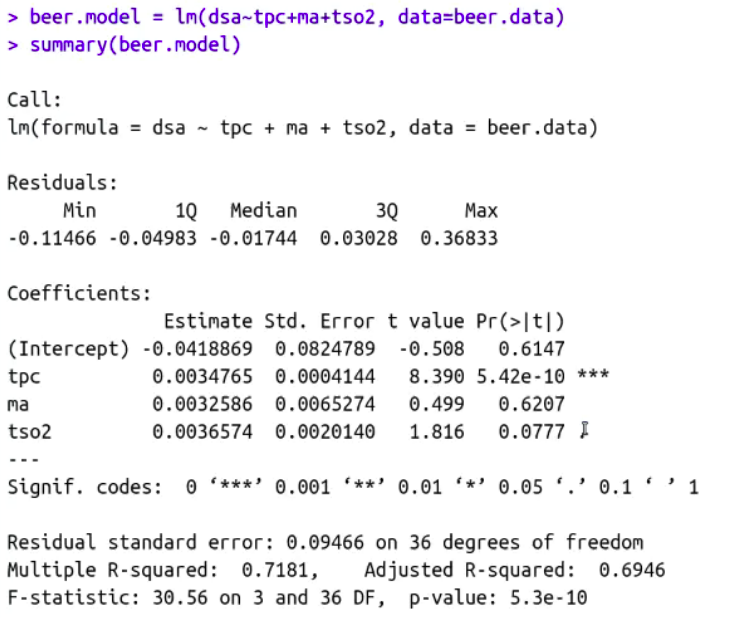
\includegraphics[scale=0.4]{images/dsa_analisis_3_variables.png}
    \caption{Captura de pantalla de los resultados del análisis DSA utilizando 3 variables}
    \label{fig:dsa_3_variables}
\end{figure}


\begin{figure}[htbp]
    \centering
    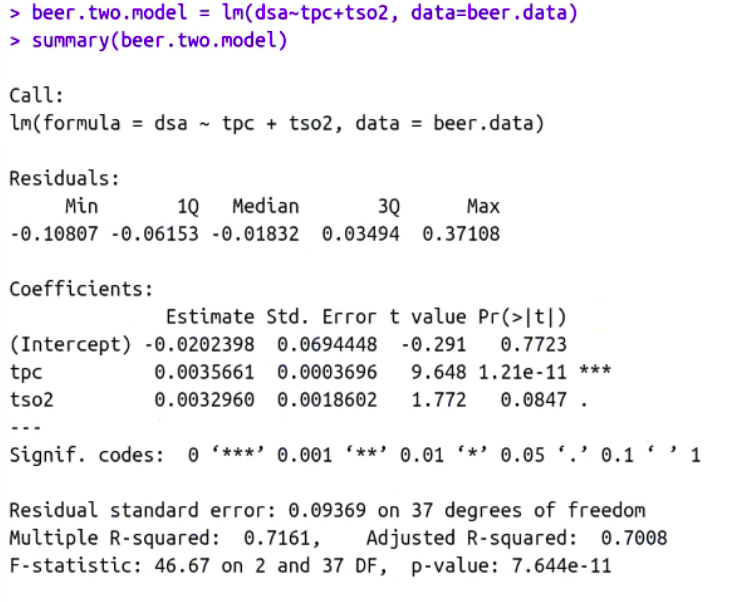
\includegraphics[scale=0.4]{images/dsa_analisis_2_variables.png}
    \caption{Captura de pantalla de los resultados del análisis DSA sin la variable \textit{ma}}
    \label{fig:dsa_2_variables}
\end{figure}


\begin{figure}[htbp]
    \centering
    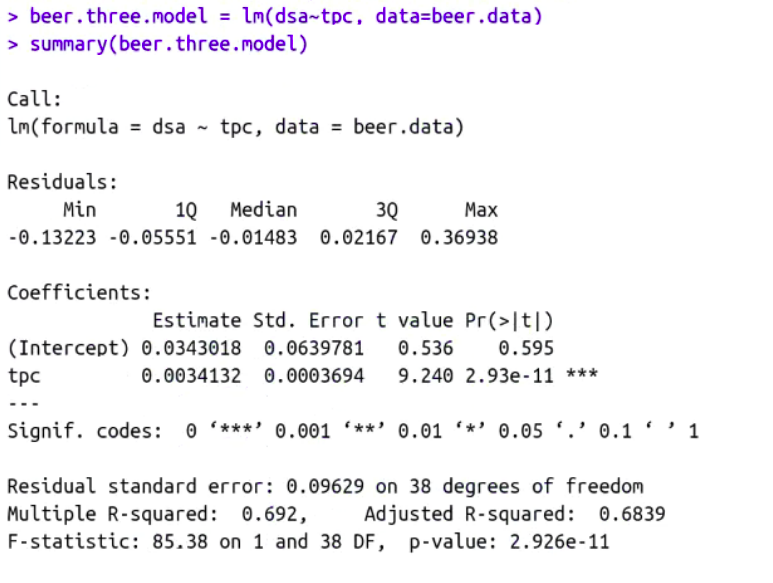
\includegraphics[scale=0.4]{images/dsa_analisis_1_variable.png}
    \caption{Captura de pantalla de los resultadolabel={lst:label}s del análisis DSA solo con la variable \textit{tpc}}
    \label{fig:dsa_1_variable}
\end{figure}


\begin{figure}[htbp]
    \centering
    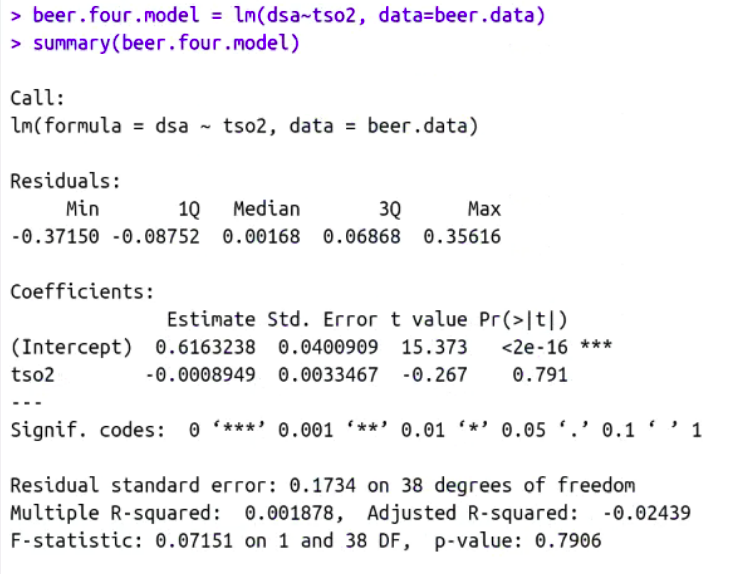
\includegraphics[scale=0.4]{images/dsa_analisis_tso2.png}
    \caption{Captura de pantalla de la salida del análisis DSA solo con la variable \textit{tso2}}
    \label{fig:dsa_1_variable_tso2}
\end{figure}


% Análisis RP
\newpage
\subsection{Análisis RP}

\begin{figure}[htbp]
    \centering
    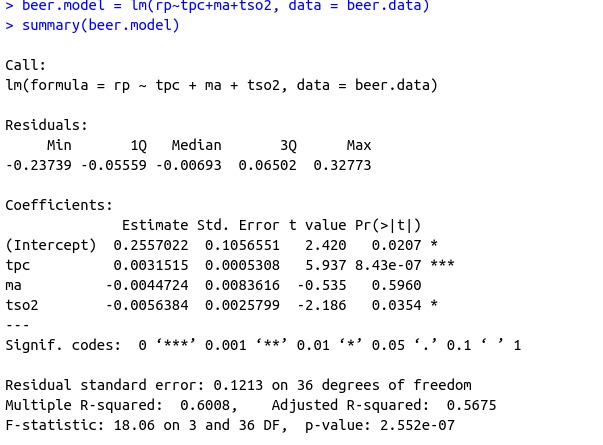
\includegraphics[scale=0.4]{images/rp_analisis_3_variables.jpeg}
    \caption{Captura de pantalla de la salida del análisis RP utilizando las 3 variables}
    \label{fig:rp_3_variables}
\end{figure}


\begin{figure}[htbp]
    \centering
    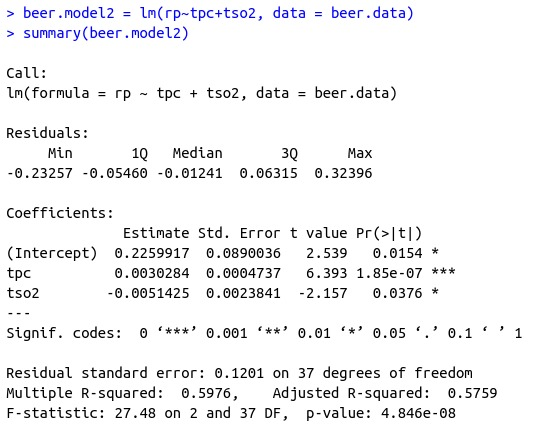
\includegraphics[scale=0.4]{images/rp_analisis_2_variables.jpeg}
    \caption{Captura de pantalla de la salida del análisis RP utilizando 2 variables (\textit{tpc} y \textit{tso2})}
    \label{fig:rp_2_variables}
\end{figure}


\begin{figure}[htbp]
    \centering
    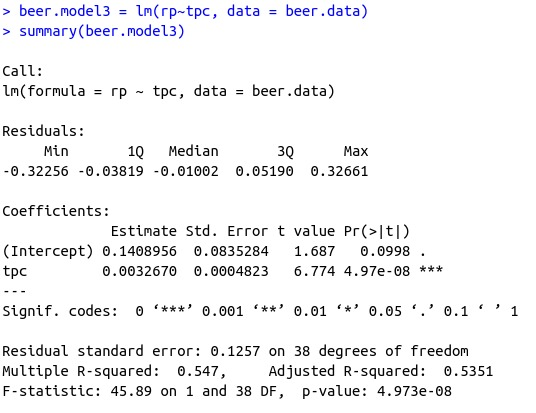
\includegraphics[scale=0.4]{images/rp_analisis_1_variable_tpc.jpeg}
    \caption{Captura de pantalla de la salida del análisis RP utilizando la variable \textit{tpc}}
    \label{fig:rp_1_variable_tpc}
\end{figure}


\begin{figure}[htbp]
    \centering
    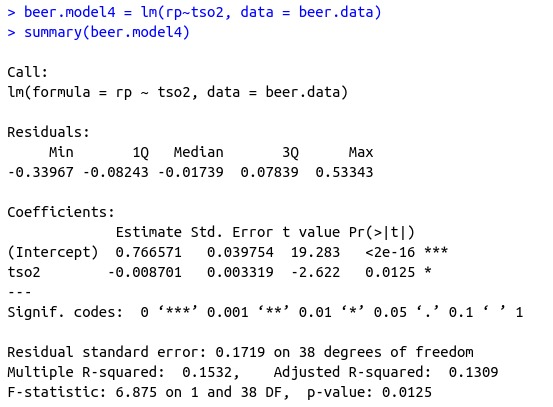
\includegraphics[scale=0.4]{images/rp_analisis_1_variable_tso2.jpeg}
    \caption{Captura de pantalla de la salida del análisis RP utilizando la variable \textit{tso2}}
    \label{fig:rp_1_variable_tso2}
\end{figure}



% Análisis ORAC
\newpage
\subsection{Análisis ORAC}
\begin{figure}[htbp]
    \centering
    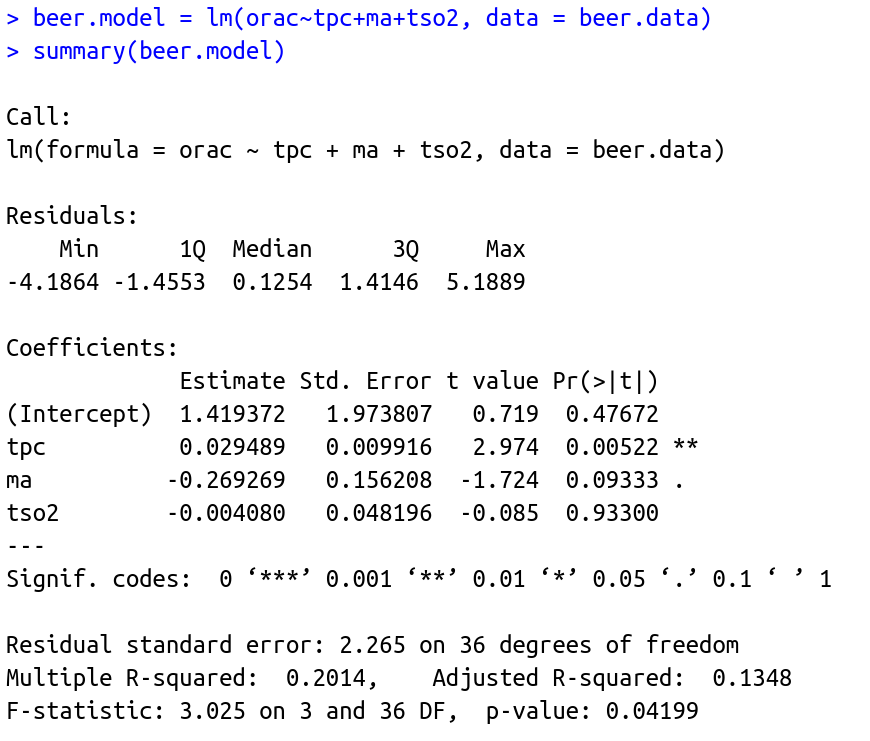
\includegraphics[scale=0.4]{images/orac_analisis_3_variables.png}
    \caption{Captura de pantalla de la salida del análisis ORAC utilizando las tres variables.}
    \label{fig:orac_3_variables}
\end{figure}

\begin{figure}[htbp]
    \centering
    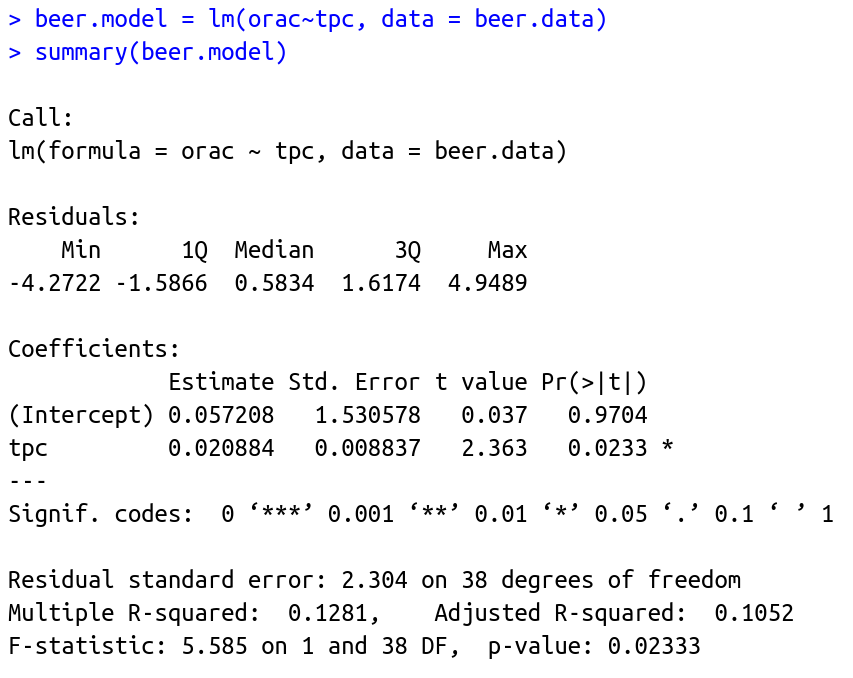
\includegraphics[scale=0.4]{images/orac_1_variable_tpc.png}
    \caption{Captura de pantalla de la salida del análisis ORAC utilizando únicamente tpc.}
    \label{fig:orac_1_variable_tpc}
\end{figure}

\begin{figure}[htbp]
    \centering
    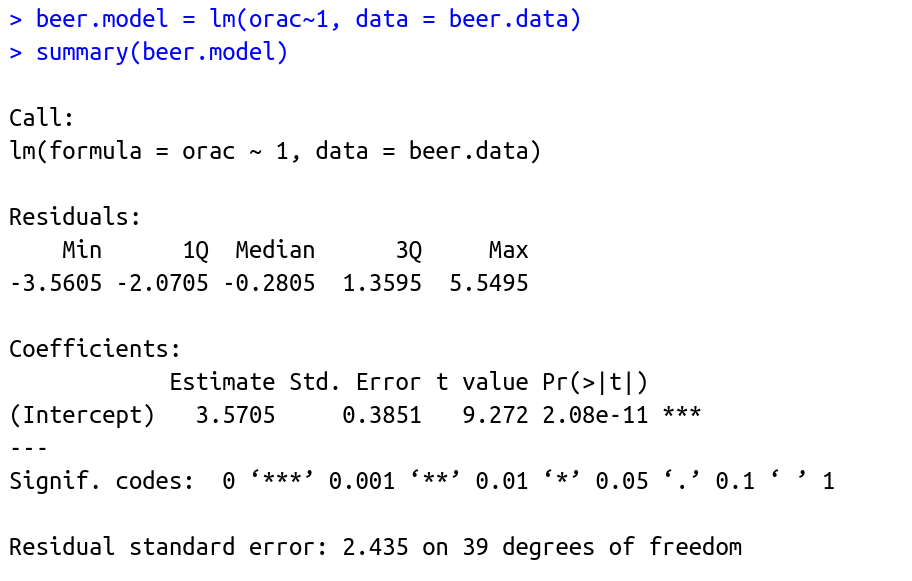
\includegraphics[scale=0.4]{images/media_orac.png}
    \caption{Captura de pantalla del análisis ORAC sin predictores.}
    \label{fig:media_orac}
\end{figure}


% Análisis ASA
\newpage
\subsection{Análisis ASA}
\begin{figure}[htbp]
    \centering
    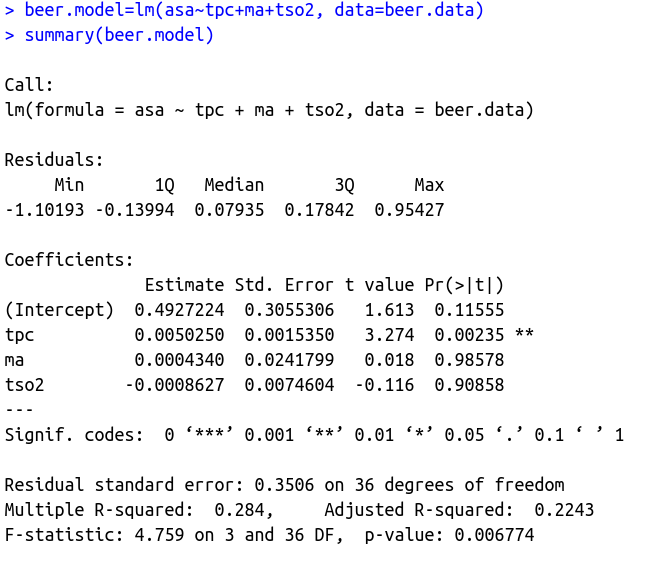
\includegraphics[scale=0.4]{images/asa_3_variables.png}
    \caption{Captura de pantalla de la salida del análisis ASA  utilizando las tres variables.}
    \label{fig:asa_3_variables}
\end{figure}

\begin{figure}[htbp]
    \centering
    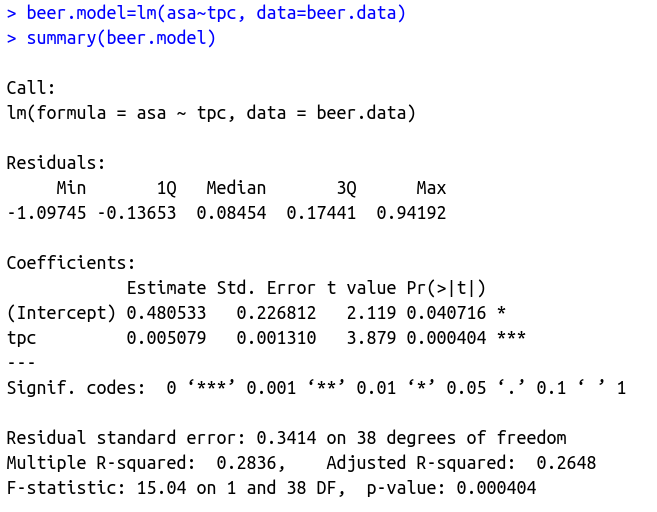
\includegraphics[scale=0.4]{images/asa_1_variable.png}
    \caption{Captura de pantalla de la salida del análisis ASA utilizando únicamente tpc.}
    \label{fig:asa_1_variable}
\end{figure}

\begin{figure}[htbp]
    \centering
    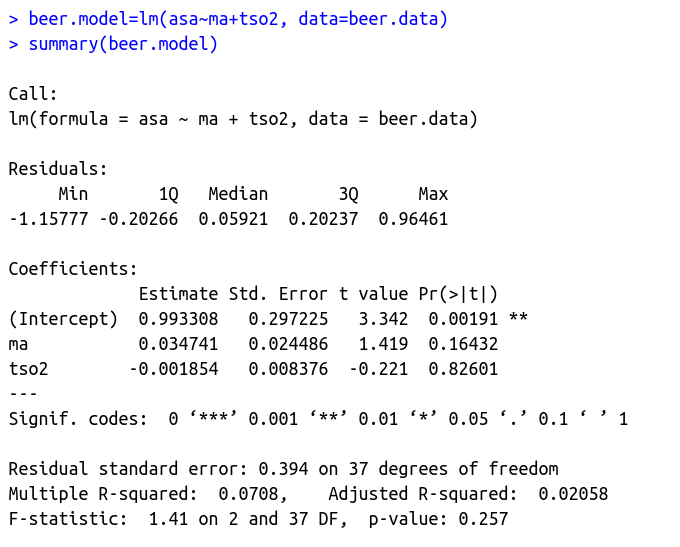
\includegraphics[scale=0.4]{images/asa_2_variables.png}
    \caption{Captura de pantalla del análisis ASA utilizando ma y tso2}
    \label{fig:asa_2_variables}
\end{figure}


% Análisis MCA
\newpage
\subsection{Análisis MCA}
\begin{figure}[htbp]
    \centering
    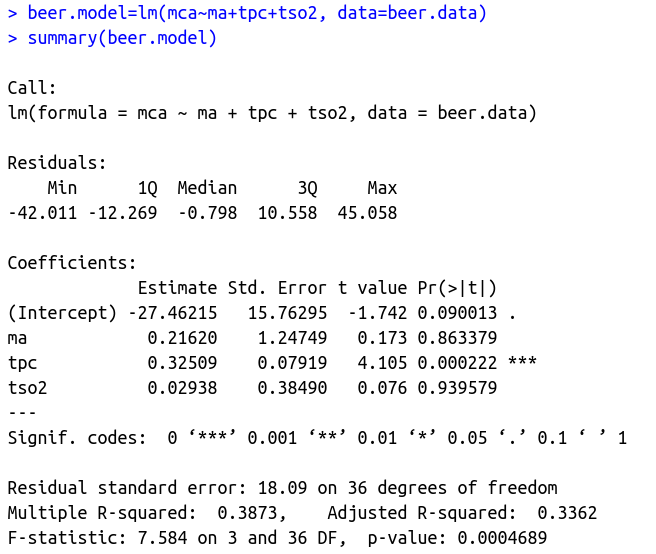
\includegraphics[scale=0.4]{images/mca_3_variables.png}
    \caption{Captura de pantalla de la salida del análisis MCA  utilizando las tres variables.}
    \label{fig:mca_3_variables}
\end{figure}


\newpage
\subsection{Análisis Modelo con longitud y latitud}
\begin{figure}[htbp]
    \centering
    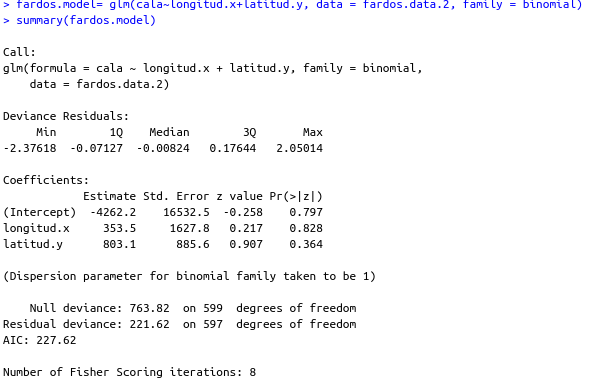
\includegraphics[scale=0.6]{images/modelo_2_param.png}
    \caption{Captura de pantalla de la salida del análisis del modelo de la playa utilizando longitud y latitud.}
    \label{fig:modelo_2_param}
\end{figure}


\newpage
\subsection{Interpretación geométrica de la división de la playa}
\begin{figure}[htbp]
    \centering
    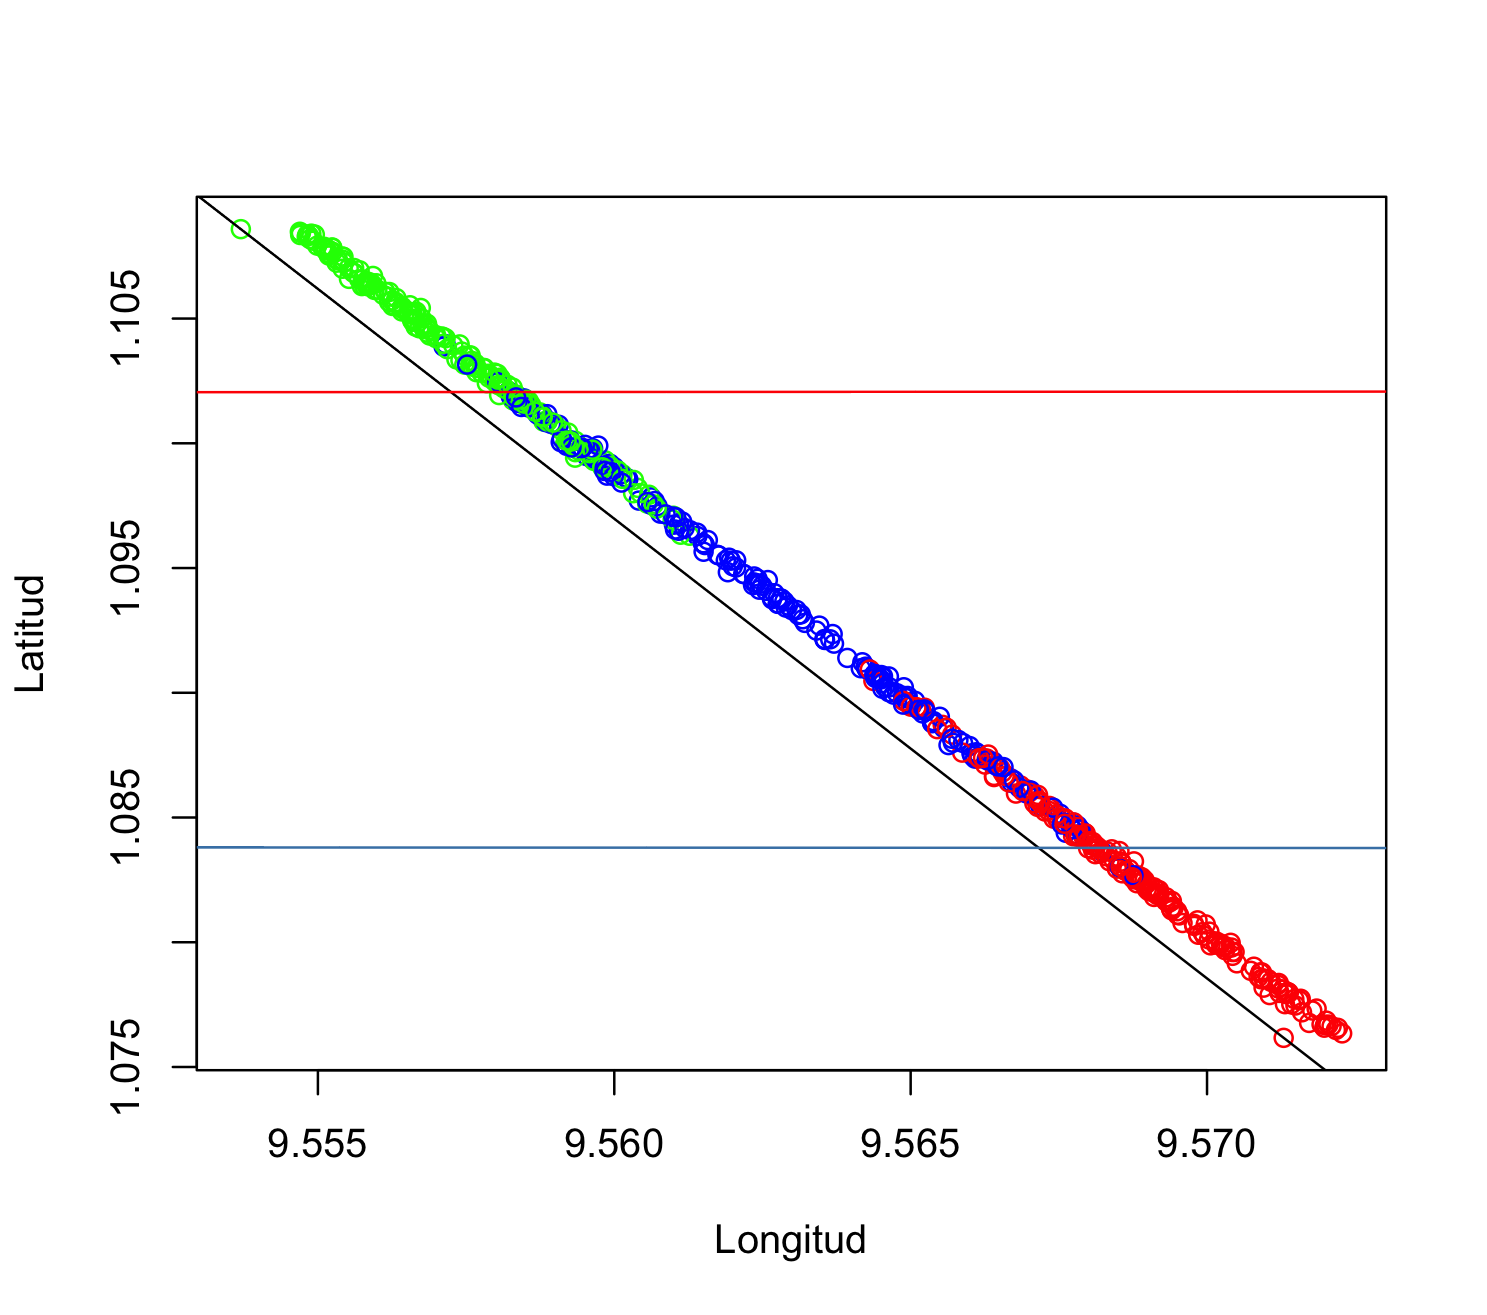
\includegraphics[scale=0.25]{images/interpretacionModelosBuenos.png}
    \caption{Interpretación geométrica de la división de la playa. En rojo: cala 2, en azul: cala 1 y en verde: cala 0. La playa queda dividida por dos rectas que intersectan con la línea formada por los fardos. Esas dos intersecciones dan como resultados los puntos norte y sur.}
    \label{fig:divisionPlayaRectas}
\end{figure}


\subsection{Matriz de confusión Parte 1}
\begin{figure}[htbp]
    \centering
    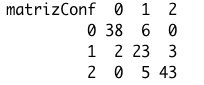
\includegraphics[scale=0.6]{images/matrizConfusion.png}
    \caption{Matriz de confusión para el modelo de la playa.}
    \label{fig:matrizConfusion}
\end{figure}


% Anexo de codigos
\newpage
\section{Anexo 2: Códigos}

\subsection{Código de creación de modelos}

\lstinputlisting[language=R, linerange={101-120}, caption={Fragmento de código de la definición de los modelos de regresión logística}, label={listing:codigoFardosModelos}]{listings/codigoFardos.R}


\newpage
\subsection{Resultados ejecución parte 2}

\begin{lstlisting}[label={lst:label}]
[1] 0.0005866667
Se podria haber hecho con 60 fardos.
Media de las peores distancias del primer punto de separacion:  501.3619 
Media de las peores distancias del segundo punto de separacion:  464.8893 
Media de los peores porcentajes de acierto:  0.8222533 
[1] 0.00349
Se podria haber hecho con 120 fardos.
Media de las peores distancias del primer punto de separacion:  297.9804 
Media de las peores distancias del segundo punto de separacion:  299.8049 
Media de los peores porcentajes de acierto:  0.8251567 
[1] 0.004413333
Se podria haber hecho con 180 fardos.
Media de las peores distancias del primer punto de separacion:  233.2526 
Media de las peores distancias del segundo punto de separacion:  221.0558 
Media de los peores porcentajes de acierto:  0.82608 
[1] 0.004885
Se podria haber hecho con 240 fardos.
Media de las peores distancias del primer punto de separacion:  178.2154 
Media de las peores distancias del segundo punto de separacion:  165.3858 
Media de los peores porcentajes de acierto:  0.8265517 
[1] 0.005021667
Se podria haber hecho con 300 fardos.
Media de las peores distancias del primer punto de separacion:  142.3178 
Media de las peores distancias del segundo punto de separacion:  136.9945 
Media de los peores porcentajes de acierto:  0.8266883 
[1] 0.0047
Se podria haber hecho con 360 fardos.
Media de las peores distancias del primer punto de separacion:  121.6917 
Media de las peores distancias del segundo punto de separacion:  109.2879 
Media de los peores porcentajes de acierto:  0.8263667 
[1] 0.00473
Se podria haber hecho con 420 fardos.
Media de las peores distancias del primer punto de separacion:  97.99388 
Media de las peores distancias del segundo punto de separacion:  94.66309 
Media de los peores porcentajes de acierto:  0.8263967 
[1] 0.004541667
Se podria haber hecho con 480 fardos.
Media de las peores distancias del primer punto de separacion:  74.27477 
Media de las peores distancias del segundo punto de separacion:  69.41352 
Media de los peores porcentajes de acierto:  0.8262083 
[1] 0.003846667
Se podria haber hecho con 540 fardos.
Media de las peores distancias del primer punto de separacion:  46.11319 
Media de las peores distancias del segundo punto de separacion:  44.92015 
Media de los peores porcentajes de acierto:  0.8255133 
\end{lstlisting}

% Bibliografía
\newpage
\addcontentsline{toc}{section}{Referencias}
\bibliographystyle{unsrt}
\bibliography{bibliografia.bib}

\end{document}